\documentclass[1p]{elsarticle_modified}
%\bibliographystyle{elsarticle-num}

%\usepackage[colorlinks]{hyperref}
%\usepackage{abbrmath_seonhwa} %\Abb, \Ascr, \Acal ,\Abf, \Afrak
\usepackage{amsfonts}
\usepackage{amssymb}
\usepackage{amsmath}
\usepackage{amsthm}
\usepackage{scalefnt}
\usepackage{amsbsy}
\usepackage{kotex}
\usepackage{caption}
\usepackage{subfig}
\usepackage{color}
\usepackage{graphicx}
\usepackage{xcolor} %% white, black, red, green, blue, cyan, magenta, yellow
\usepackage{float}
\usepackage{setspace}
\usepackage{hyperref}

\usepackage{tikz}
\usetikzlibrary{arrows}

\usepackage{multirow}
\usepackage{array} % fixed length table
\usepackage{hhline}

%%%%%%%%%%%%%%%%%%%%%
\makeatletter
\renewcommand*\env@matrix[1][\arraystretch]{%
	\edef\arraystretch{#1}%
	\hskip -\arraycolsep
	\let\@ifnextchar\new@ifnextchar
	\array{*\c@MaxMatrixCols c}}
\makeatother %https://tex.stackexchange.com/questions/14071/how-can-i-increase-the-line-spacing-in-a-matrix
%%%%%%%%%%%%%%%

\usepackage[normalem]{ulem}

\newcommand{\msout}[1]{\ifmmode\text{\sout{\ensuremath{#1}}}\else\sout{#1}\fi}
%SOURCE: \msout is \stkout macro in https://tex.stackexchange.com/questions/20609/strikeout-in-math-mode

\newcommand{\cancel}[1]{
	\ifmmode
	{\color{red}\msout{#1}}
	\else
	{\color{red}\sout{#1}}
	\fi
}

\newcommand{\add}[1]{
	{\color{blue}\uwave{#1}}
}

\newcommand{\replace}[2]{
	\ifmmode
	{\color{red}\msout{#1}}{\color{blue}\uwave{#2}}
	\else
	{\color{red}\sout{#1}}{\color{blue}\uwave{#2}}
	\fi
}

\newcommand{\Sol}{\mathcal{S}} %segment
\newcommand{\D}{D} %diagram
\newcommand{\A}{\mathcal{A}} %arc


%%%%%%%%%%%%%%%%%%%%%%%%%%%%%5 test

\def\sl{\operatorname{\textup{SL}}(2,\Cbb)}
\def\psl{\operatorname{\textup{PSL}}(2,\Cbb)}
\def\quan{\mkern 1mu \triangleright \mkern 1mu}

\theoremstyle{definition}
\newtheorem{thm}{Theorem}[section]
\newtheorem{prop}[thm]{Proposition}
\newtheorem{lem}[thm]{Lemma}
\newtheorem{ques}[thm]{Question}
\newtheorem{cor}[thm]{Corollary}
\newtheorem{defn}[thm]{Definition}
\newtheorem{exam}[thm]{Example}
\newtheorem{rmk}[thm]{Remark}
\newtheorem{alg}[thm]{Algorithm}

\newcommand{\I}{\sqrt{-1}}
\begin{document}

%\begin{frontmatter}
%
%\title{Boundary parabolic representations of knots up to 8 crossings}
%
%%% Group authors per affiliation:
%\author{Yunhi Cho} 
%\address{Department of Mathematics, University of Seoul, Seoul, Korea}
%\ead{yhcho@uos.ac.kr}
%
%
%\author{Seonhwa Kim} %\fnref{s_kim}}
%\address{Center for Geometry and Physics, Institute for Basic Science, Pohang, 37673, Korea}
%\ead{ryeona17@ibs.re.kr}
%
%\author{Hyuk Kim}
%\address{Department of Mathematical Sciences, Seoul National University, Seoul 08826, Korea}
%\ead{hyukkim@snu.ac.kr}
%
%\author{Seokbeom Yoon}
%\address{Department of Mathematical Sciences, Seoul National University, Seoul, 08826,  Korea}
%\ead{sbyoon15@snu.ac.kr}
%
%\begin{abstract}
%We find all boundary parabolic representation of knots up to 8 crossings.
%
%\end{abstract}
%\begin{keyword}
%    \MSC[2010] 57M25 
%\end{keyword}
%
%\end{frontmatter}

%\linenumbers
%\tableofcontents
%
\newcommand\colored[1]{\textcolor{white}{\rule[-0.35ex]{0.8em}{1.4ex}}\kern-0.8em\color{red} #1}%
%\newcommand\colored[1]{\textcolor{white}{ #1}\kern-2.17ex	\textcolor{white}{ #1}\kern-1.81ex	\textcolor{white}{ #1}\kern-2.15ex\color{red}#1	}

{\Large $\underline{11a_{300}~(K11a_{300})}$}

\setlength{\tabcolsep}{10pt}
\renewcommand{\arraystretch}{1.6}
\vspace{1cm}\begin{tabular}{m{100pt}>{\centering\arraybackslash}m{274pt}}
\multirow{5}{120pt}{
	\centering
	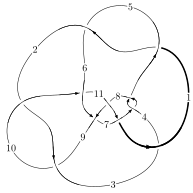
\includegraphics[width=112pt]{../../../GIT/diagram.site/Diagrams/png/549_11a_300.png}\\
\ \ \ A knot diagram\footnotemark}&
\allowdisplaybreaks
\textbf{Linearized knot diagam} \\
\cline{2-2}
 &
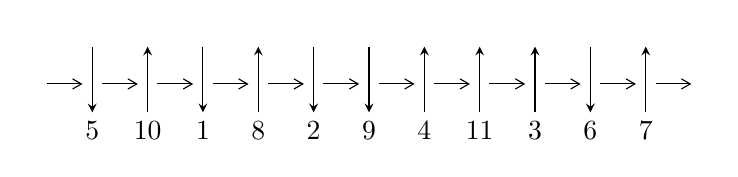
\begin{tikzpicture}[x=20pt, y=17pt]
	% nodes
	\node (C0) at (0, 0) {};
	\node (C1) at (1, 0) {};
	\node (C1U) at (1, +1) {};
	\node (C1D) at (1, -1) {5};

	\node (C2) at (2, 0) {};
	\node (C2U) at (2, +1) {};
	\node (C2D) at (2, -1) {10};

	\node (C3) at (3, 0) {};
	\node (C3U) at (3, +1) {};
	\node (C3D) at (3, -1) {1};

	\node (C4) at (4, 0) {};
	\node (C4U) at (4, +1) {};
	\node (C4D) at (4, -1) {8};

	\node (C5) at (5, 0) {};
	\node (C5U) at (5, +1) {};
	\node (C5D) at (5, -1) {2};

	\node (C6) at (6, 0) {};
	\node (C6U) at (6, +1) {};
	\node (C6D) at (6, -1) {9};

	\node (C7) at (7, 0) {};
	\node (C7U) at (7, +1) {};
	\node (C7D) at (7, -1) {4};

	\node (C8) at (8, 0) {};
	\node (C8U) at (8, +1) {};
	\node (C8D) at (8, -1) {11};

	\node (C9) at (9, 0) {};
	\node (C9U) at (9, +1) {};
	\node (C9D) at (9, -1) {3};

	\node (C10) at (10, 0) {};
	\node (C10U) at (10, +1) {};
	\node (C10D) at (10, -1) {6};

	\node (C11) at (11, 0) {};
	\node (C11U) at (11, +1) {};
	\node (C11D) at (11, -1) {7};
	\node (C12) at (12, 0) {};

	% arrows
	\draw[->,>={angle 60}]
	(C0) edge (C1) (C1) edge (C2) (C2) edge (C3) (C3) edge (C4) (C4) edge (C5) (C5) edge (C6) (C6) edge (C7) (C7) edge (C8) (C8) edge (C9) (C9) edge (C10) (C10) edge (C11) (C11) edge (C12) ;	\draw[->,>=stealth]
	(C1U) edge (C1D) (C2D) edge (C2U) (C3U) edge (C3D) (C4D) edge (C4U) (C5U) edge (C5D) (C6U) edge (C6D) (C7D) edge (C7U) (C8D) edge (C8U) (C9D) edge (C9U) (C10U) edge (C10D) (C11D) edge (C11U) ;
	\end{tikzpicture} \\
\hhline{~~} \\& 
\textbf{Solving Sequence} \\ \cline{2-2} 
 &
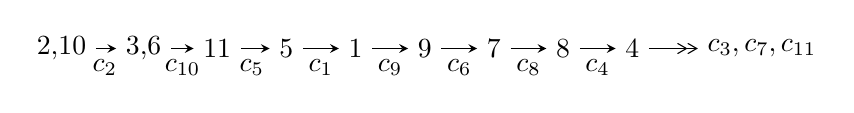
\begin{tikzpicture}[x=25pt, y=7pt]
	% node
	\node (A0) at (-1/8, 0) {2,10};
	\node (A1) at (17/16, 0) {3,6};
	\node (A2) at (17/8, 0) {11};
	\node (A3) at (25/8, 0) {5};
	\node (A4) at (33/8, 0) {1};
	\node (A5) at (41/8, 0) {9};
	\node (A6) at (49/8, 0) {7};
	\node (A7) at (57/8, 0) {8};
	\node (A8) at (65/8, 0) {4};
	\node (C1) at (1/2, -1) {$c_{2}$};
	\node (C2) at (13/8, -1) {$c_{10}$};
	\node (C3) at (21/8, -1) {$c_{5}$};
	\node (C4) at (29/8, -1) {$c_{1}$};
	\node (C5) at (37/8, -1) {$c_{9}$};
	\node (C6) at (45/8, -1) {$c_{6}$};
	\node (C7) at (53/8, -1) {$c_{8}$};
	\node (C8) at (61/8, -1) {$c_{4}$};
	\node (A9) at (10, 0) {$c_{3},c_{7},c_{11}$};

	% edge
	\draw[->,>=stealth]	
	(A0) edge (A1) (A1) edge (A2) (A2) edge (A3) (A3) edge (A4) (A4) edge (A5) (A5) edge (A6) (A6) edge (A7) (A7) edge (A8) ;
	\draw[->>,>={angle 60}]	
	(A8) edge (A9);
\end{tikzpicture} \\ 

\end{tabular} \\

\footnotetext{
The image of knot diagram is generated by the software ``\textbf{Draw programme}" developed by Andrew Bartholomew(\url{http://www.layer8.co.uk/maths/draw/index.htm\#Running-draw}), where we modified some parts for our purpose(\url{https://github.com/CATsTAILs/LinksPainter}).
}\phantom \\ \newline 
\centering \textbf{Ideals for irreducible components\footnotemark of $X_{\text{par}}$} 
 
\begin{align*}
I^u_{1}&=\langle 
1.10239\times10^{271} u^{95}-1.29227\times10^{272} u^{94}+\cdots+1.23928\times10^{271} b+2.12022\times10^{274},\\
\phantom{I^u_{1}}&\phantom{= \langle  }1.69259\times10^{274} u^{95}-4.36720\times10^{274} u^{94}+\cdots+2.39182\times10^{273} a+6.71018\times10^{276},\\
\phantom{I^u_{1}}&\phantom{= \langle  }u^{96}+32 u^{94}+\cdots-1260 u-193\rangle \\
I^u_{2}&=\langle 
-312425 u^{19}-462214 u^{18}+\cdots+208363 b-52657,\\
\phantom{I^u_{2}}&\phantom{= \langle  }2692148 u^{19}+2660136 u^{18}+\cdots+1041815 a+3674309,\;u^{20}+u^{19}+\cdots+2 u-1\rangle \\
\\
\end{align*}
\raggedright * 2 irreducible components of $\dim_{\mathbb{C}}=0$, with total 116 representations.\\
\footnotetext{All coefficients of polynomials are rational numbers. But the coefficients are sometimes approximated in decimal forms when there is not enough margin.}
\newpage
\renewcommand{\arraystretch}{1}
\centering \section*{I. $I^u_{1}= \langle 1.10\times10^{271} u^{95}-1.29\times10^{272} u^{94}+\cdots+1.24\times10^{271} b+2.12\times10^{274},\;1.69\times10^{274} u^{95}-4.37\times10^{274} u^{94}+\cdots+2.39\times10^{273} a+6.71\times10^{276},\;u^{96}+32 u^{94}+\cdots-1260 u-193 \rangle$}
\flushleft \textbf{(i) Arc colorings}\\
\begin{tabular}{m{7pt} m{180pt} m{7pt} m{180pt} }
\flushright $a_{2}=$&$\begin{pmatrix}1\\0\end{pmatrix}$ \\
\flushright $a_{10}=$&$\begin{pmatrix}0\\u\end{pmatrix}$ \\
\flushright $a_{3}=$&$\begin{pmatrix}1\\- u^2\end{pmatrix}$ \\
\flushright $a_{6}=$&$\begin{pmatrix}-7.07659 u^{95}+18.2589 u^{94}+\cdots-16539.3 u-2805.47\\-0.889541 u^{95}+10.4276 u^{94}+\cdots-10657.3 u-1710.84\end{pmatrix}$ \\
\flushright $a_{11}=$&$\begin{pmatrix}-7.96908 u^{95}+10.7719 u^{94}+\cdots-8088.81 u-1484.13\\0.381477 u^{95}+4.65214 u^{94}+\cdots-5016.46 u-782.330\end{pmatrix}$ \\
\flushright $a_{5}=$&$\begin{pmatrix}-7.96613 u^{95}+28.6864 u^{94}+\cdots-27196.6 u-4516.31\\-0.889541 u^{95}+10.4276 u^{94}+\cdots-10657.3 u-1710.84\end{pmatrix}$ \\
\flushright $a_{1}=$&$\begin{pmatrix}-4.42194 u^{95}+1.59863 u^{94}+\cdots-63.9621 u-122.087\\-0.368419 u^{95}+1.21715 u^{94}+\cdots-1301.07 u-213.070\end{pmatrix}$ \\
\flushright $a_{9}=$&$\begin{pmatrix}- u\\u^3+u\end{pmatrix}$ \\
\flushright $a_{7}=$&$\begin{pmatrix}-10.1408 u^{95}+26.9593 u^{94}+\cdots-24457.0 u-4141.68\\0.821675 u^{95}+12.0458 u^{94}+\cdots-13110.7 u-2053.80\end{pmatrix}$ \\
\flushright $a_{8}=$&$\begin{pmatrix}24.0257 u^{95}-8.64454 u^{94}+\cdots-603.693 u+534.594\\6.39239 u^{95}-8.97364 u^{94}+\cdots+6887.06 u+1253.19\end{pmatrix}$ \\
\flushright $a_{4}=$&$\begin{pmatrix}-23.1189 u^{95}+9.51320 u^{94}+\cdots-721.295 u-719.317\\-6.76103 u^{95}+8.21702 u^{94}+\cdots-5918.27 u-1108.98\end{pmatrix}$\\ \flushright $a_{4}=$&$\begin{pmatrix}-23.1189 u^{95}+9.51320 u^{94}+\cdots-721.295 u-719.317\\-6.76103 u^{95}+8.21702 u^{94}+\cdots-5918.27 u-1108.98\end{pmatrix}$\\&\end{tabular}
\flushleft \textbf{(ii) Obstruction class $= -1$}\\~\\
\flushleft \textbf{(iii) Cusp Shapes $= 7.10864 u^{95}+21.6510 u^{94}+\cdots-27025.5 u-4094.60$}\\~\\
\newpage\renewcommand{\arraystretch}{1}
\flushleft \textbf{(iv) u-Polynomials at the component}\newline \\
\begin{tabular}{m{50pt}|m{274pt}}
Crossings & \hspace{64pt}u-Polynomials at each crossing \\
\hline $$\begin{aligned}c_{1},c_{5}\end{aligned}$$&$\begin{aligned}
&u^{96}- u^{95}+\cdots+44434 u+5239
\end{aligned}$\\
\hline $$\begin{aligned}c_{2},c_{9}\end{aligned}$$&$\begin{aligned}
&u^{96}+32 u^{94}+\cdots-1260 u-193
\end{aligned}$\\
\hline $$\begin{aligned}c_{3}\end{aligned}$$&$\begin{aligned}
&u^{96}-9 u^{95}+\cdots+371 u-46
\end{aligned}$\\
\hline $$\begin{aligned}c_{4},c_{7}\end{aligned}$$&$\begin{aligned}
&u^{96}+u^{95}+\cdots+60 u-101
\end{aligned}$\\
\hline $$\begin{aligned}c_{6}\end{aligned}$$&$\begin{aligned}
&u^{96}-4 u^{95}+\cdots-45 u+1
\end{aligned}$\\
\hline $$\begin{aligned}c_{8}\end{aligned}$$&$\begin{aligned}
&u^{96}+10 u^{95}+\cdots+3240 u+368
\end{aligned}$\\
\hline $$\begin{aligned}c_{10}\end{aligned}$$&$\begin{aligned}
&u^{96}+2 u^{95}+\cdots-159407 u-226723
\end{aligned}$\\
\hline $$\begin{aligned}c_{11}\end{aligned}$$&$\begin{aligned}
&u^{96}-6 u^{95}+\cdots-14458 u+1789
\end{aligned}$\\
\hline
\end{tabular}\\~\\
\newpage\renewcommand{\arraystretch}{1}
\flushleft \textbf{(v) Riley Polynomials at the component}\newline \\
\begin{tabular}{m{50pt}|m{274pt}}
Crossings & \hspace{64pt}Riley Polynomials at each crossing \\
\hline $$\begin{aligned}c_{1},c_{5}\end{aligned}$$&$\begin{aligned}
&y^{96}-73 y^{95}+\cdots+553636226 y+27447121
\end{aligned}$\\
\hline $$\begin{aligned}c_{2},c_{9}\end{aligned}$$&$\begin{aligned}
&y^{96}+64 y^{95}+\cdots+1764038 y+37249
\end{aligned}$\\
\hline $$\begin{aligned}c_{3}\end{aligned}$$&$\begin{aligned}
&y^{96}- y^{95}+\cdots+405435 y+2116
\end{aligned}$\\
\hline $$\begin{aligned}c_{4},c_{7}\end{aligned}$$&$\begin{aligned}
&y^{96}-53 y^{95}+\cdots-127426 y+10201
\end{aligned}$\\
\hline $$\begin{aligned}c_{6}\end{aligned}$$&$\begin{aligned}
&y^{96}-4 y^{95}+\cdots-559 y+1
\end{aligned}$\\
\hline $$\begin{aligned}c_{8}\end{aligned}$$&$\begin{aligned}
&y^{96}-10 y^{95}+\cdots+3636544 y+135424
\end{aligned}$\\
\hline $$\begin{aligned}c_{10}\end{aligned}$$&$\begin{aligned}
&y^{96}-36 y^{95}+\cdots-374201254849 y+51403318729
\end{aligned}$\\
\hline $$\begin{aligned}c_{11}\end{aligned}$$&$\begin{aligned}
&y^{96}-16 y^{95}+\cdots-110849866 y+3200521
\end{aligned}$\\
\hline
\end{tabular}\\~\\
\newpage\flushleft \textbf{(vi) Complex Volumes and Cusp Shapes}
$$\begin{array}{c|c|c}  
\text{Solutions to }I^u_{1}& \I (\text{vol} + \sqrt{-1}CS) & \text{Cusp shape}\\
 \hline 
\begin{aligned}
u &= \phantom{-}0.477710 + 0.871860 I \\
a &= -1.58702 + 0.33319 I \\
b &= \phantom{-}0.579139 + 0.546384 I\end{aligned}
 & \phantom{-}1.89831 + 4.86756 I & \phantom{-0.000000 } 0 \\ \hline\begin{aligned}
u &= \phantom{-}0.477710 - 0.871860 I \\
a &= -1.58702 - 0.33319 I \\
b &= \phantom{-}0.579139 - 0.546384 I\end{aligned}
 & \phantom{-}1.89831 - 4.86756 I & \phantom{-0.000000 } 0 \\ \hline\begin{aligned}
u &= \phantom{-}0.349612 + 0.927401 I \\
a &= \phantom{-}0.028575 + 0.982383 I \\
b &= \phantom{-}0.443823 - 0.618828 I\end{aligned}
 & -0.40537 + 1.96180 I & \phantom{-0.000000 } 0 \\ \hline\begin{aligned}
u &= \phantom{-}0.349612 - 0.927401 I \\
a &= \phantom{-}0.028575 - 0.982383 I \\
b &= \phantom{-}0.443823 + 0.618828 I\end{aligned}
 & -0.40537 - 1.96180 I & \phantom{-0.000000 } 0 \\ \hline\begin{aligned}
u &= -0.150164 + 1.021670 I \\
a &= \phantom{-}1.31047 + 0.62522 I \\
b &= \phantom{-}0.801587 - 0.111152 I\end{aligned}
 & \phantom{-}0.829229 + 0.160481 I & \phantom{-0.000000 } 0 \\ \hline\begin{aligned}
u &= -0.150164 - 1.021670 I \\
a &= \phantom{-}1.31047 - 0.62522 I \\
b &= \phantom{-}0.801587 + 0.111152 I\end{aligned}
 & \phantom{-}0.829229 - 0.160481 I & \phantom{-0.000000 } 0 \\ \hline\begin{aligned}
u &= -0.006380 + 0.958245 I \\
a &= -0.372426 + 0.041323 I \\
b &= -2.84025 + 2.76183 I\end{aligned}
 & -1.83794 + 0.18273 I & \phantom{-0.000000 } 0 \\ \hline\begin{aligned}
u &= -0.006380 - 0.958245 I \\
a &= -0.372426 - 0.041323 I \\
b &= -2.84025 - 2.76183 I\end{aligned}
 & -1.83794 - 0.18273 I & \phantom{-0.000000 } 0 \\ \hline\begin{aligned}
u &= \phantom{-}1.006110 + 0.273433 I \\
a &= \phantom{-}0.044883 - 0.674284 I \\
b &= -0.402873 + 0.524513 I\end{aligned}
 & \phantom{-}5.03978 + 1.15243 I & \phantom{-0.000000 } 0 \\ \hline\begin{aligned}
u &= \phantom{-}1.006110 - 0.273433 I \\
a &= \phantom{-}0.044883 + 0.674284 I \\
b &= -0.402873 - 0.524513 I\end{aligned}
 & \phantom{-}5.03978 - 1.15243 I & \phantom{-0.000000 } 0\\
 \hline 
 \end{array}$$\newpage$$\begin{array}{c|c|c}  
\text{Solutions to }I^u_{1}& \I (\text{vol} + \sqrt{-1}CS) & \text{Cusp shape}\\
 \hline 
\begin{aligned}
u &= \phantom{-}0.762249 + 0.575493 I \\
a &= \phantom{-}1.147770 - 0.749601 I \\
b &= -1.101860 + 0.348699 I\end{aligned}
 & \phantom{-}0.74726 + 5.71599 I & \phantom{-0.000000 } 0 \\ \hline\begin{aligned}
u &= \phantom{-}0.762249 - 0.575493 I \\
a &= \phantom{-}1.147770 + 0.749601 I \\
b &= -1.101860 - 0.348699 I\end{aligned}
 & \phantom{-}0.74726 - 5.71599 I & \phantom{-0.000000 } 0 \\ \hline\begin{aligned}
u &= -0.115793 + 1.054130 I \\
a &= -1.68582 + 0.13770 I \\
b &= -1.214340 - 0.076228 I\end{aligned}
 & -2.85619 - 3.24531 I & \phantom{-0.000000 } 0 \\ \hline\begin{aligned}
u &= -0.115793 - 1.054130 I \\
a &= -1.68582 - 0.13770 I \\
b &= -1.214340 + 0.076228 I\end{aligned}
 & -2.85619 + 3.24531 I & \phantom{-0.000000 } 0 \\ \hline\begin{aligned}
u &= -0.119486 + 1.065540 I \\
a &= \phantom{-}2.23374 + 0.04464 I \\
b &= \phantom{-}1.151510 + 0.250704 I\end{aligned}
 & -0.00337 - 7.83254 I & \phantom{-0.000000 } 0 \\ \hline\begin{aligned}
u &= -0.119486 - 1.065540 I \\
a &= \phantom{-}2.23374 - 0.04464 I \\
b &= \phantom{-}1.151510 - 0.250704 I\end{aligned}
 & -0.00337 + 7.83254 I & \phantom{-0.000000 } 0 \\ \hline\begin{aligned}
u &= -0.096656 + 1.073260 I \\
a &= -0.78866 + 1.19330 I \\
b &= -1.48118 - 0.18409 I\end{aligned}
 & -5.22833 - 2.70073 I & \phantom{-0.000000 } 0 \\ \hline\begin{aligned}
u &= -0.096656 - 1.073260 I \\
a &= -0.78866 - 1.19330 I \\
b &= -1.48118 + 0.18409 I\end{aligned}
 & -5.22833 + 2.70073 I & \phantom{-0.000000 } 0 \\ \hline\begin{aligned}
u &= \phantom{-}0.101676 + 1.075690 I \\
a &= \phantom{-}0.444887 + 0.616934 I \\
b &= \phantom{-}0.67291 - 1.62907 I\end{aligned}
 & -0.605747 - 0.447290 I & \phantom{-0.000000 } 0 \\ \hline\begin{aligned}
u &= \phantom{-}0.101676 - 1.075690 I \\
a &= \phantom{-}0.444887 - 0.616934 I \\
b &= \phantom{-}0.67291 + 1.62907 I\end{aligned}
 & -0.605747 + 0.447290 I & \phantom{-0.000000 } 0\\
 \hline 
 \end{array}$$\newpage$$\begin{array}{c|c|c}  
\text{Solutions to }I^u_{1}& \I (\text{vol} + \sqrt{-1}CS) & \text{Cusp shape}\\
 \hline 
\begin{aligned}
u &= -0.083330 + 1.113740 I \\
a &= \phantom{-}0.141414 - 1.204450 I \\
b &= \phantom{-}1.263970 + 0.294772 I\end{aligned}
 & -5.35019 + 1.42280 I & \phantom{-0.000000 } 0 \\ \hline\begin{aligned}
u &= -0.083330 - 1.113740 I \\
a &= \phantom{-}0.141414 + 1.204450 I \\
b &= \phantom{-}1.263970 - 0.294772 I\end{aligned}
 & -5.35019 - 1.42280 I & \phantom{-0.000000 } 0 \\ \hline\begin{aligned}
u &= -0.861117 + 0.059028 I \\
a &= -1.101960 - 0.399619 I \\
b &= \phantom{-}1.322520 + 0.148419 I\end{aligned}
 & -3.40821 - 0.60971 I & \phantom{-0.000000 } 0 \\ \hline\begin{aligned}
u &= -0.861117 - 0.059028 I \\
a &= -1.101960 + 0.399619 I \\
b &= \phantom{-}1.322520 - 0.148419 I\end{aligned}
 & -3.40821 + 0.60971 I & \phantom{-0.000000 } 0 \\ \hline\begin{aligned}
u &= \phantom{-}0.463157 + 0.690308 I \\
a &= \phantom{-}1.207050 + 0.428007 I \\
b &= -0.160459 - 0.467180 I\end{aligned}
 & \phantom{-}0.39402 + 1.56177 I & \phantom{-0.000000 } 0 \\ \hline\begin{aligned}
u &= \phantom{-}0.463157 - 0.690308 I \\
a &= \phantom{-}1.207050 - 0.428007 I \\
b &= -0.160459 + 0.467180 I\end{aligned}
 & \phantom{-}0.39402 - 1.56177 I & \phantom{-0.000000 } 0 \\ \hline\begin{aligned}
u &= \phantom{-}0.763821 + 0.888138 I \\
a &= -0.929808 + 0.763951 I \\
b &= \phantom{-}1.044250 - 0.014042 I\end{aligned}
 & -0.0489695 - 0.0733989 I & \phantom{-0.000000 } 0 \\ \hline\begin{aligned}
u &= \phantom{-}0.763821 - 0.888138 I \\
a &= -0.929808 - 0.763951 I \\
b &= \phantom{-}1.044250 + 0.014042 I\end{aligned}
 & -0.0489695 + 0.0733989 I & \phantom{-0.000000 } 0 \\ \hline\begin{aligned}
u &= \phantom{-}0.036681 + 1.172390 I \\
a &= -0.282225 - 0.846664 I \\
b &= \phantom{-}0.382233 + 0.654066 I\end{aligned}
 & -3.96883 + 1.64207 I & \phantom{-0.000000 } 0 \\ \hline\begin{aligned}
u &= \phantom{-}0.036681 - 1.172390 I \\
a &= -0.282225 + 0.846664 I \\
b &= \phantom{-}0.382233 - 0.654066 I\end{aligned}
 & -3.96883 - 1.64207 I & \phantom{-0.000000 } 0\\
 \hline 
 \end{array}$$\newpage$$\begin{array}{c|c|c}  
\text{Solutions to }I^u_{1}& \I (\text{vol} + \sqrt{-1}CS) & \text{Cusp shape}\\
 \hline 
\begin{aligned}
u &= -0.745178 + 0.342343 I \\
a &= -0.642571 + 0.754957 I \\
b &= -0.686324 - 0.574204 I\end{aligned}
 & \phantom{-}4.50509 - 2.67262 I & \phantom{-0.000000 } 0 \\ \hline\begin{aligned}
u &= -0.745178 - 0.342343 I \\
a &= -0.642571 - 0.754957 I \\
b &= -0.686324 + 0.574204 I\end{aligned}
 & \phantom{-}4.50509 + 2.67262 I & \phantom{-0.000000 } 0 \\ \hline\begin{aligned}
u &= -0.344626 + 1.155090 I \\
a &= \phantom{-}0.053249 + 0.640010 I \\
b &= \phantom{-}0.391099 - 1.075970 I\end{aligned}
 & \phantom{-}1.96286 - 1.30339 I & \phantom{-0.000000 } 0 \\ \hline\begin{aligned}
u &= -0.344626 - 1.155090 I \\
a &= \phantom{-}0.053249 - 0.640010 I \\
b &= \phantom{-}0.391099 + 1.075970 I\end{aligned}
 & \phantom{-}1.96286 + 1.30339 I & \phantom{-0.000000 } 0 \\ \hline\begin{aligned}
u &= -0.780859 + 0.010223 I \\
a &= \phantom{-}1.36580 - 0.70315 I \\
b &= -1.178590 + 0.396139 I\end{aligned}
 & -2.44931 + 4.41382 I & \phantom{-0.000000 } 0 \\ \hline\begin{aligned}
u &= -0.780859 - 0.010223 I \\
a &= \phantom{-}1.36580 + 0.70315 I \\
b &= -1.178590 - 0.396139 I\end{aligned}
 & -2.44931 - 4.41382 I & \phantom{-0.000000 } 0 \\ \hline\begin{aligned}
u &= -0.735809 + 0.256765 I \\
a &= -1.18724 + 0.94156 I \\
b &= -0.007951 - 0.889298 I\end{aligned}
 & \phantom{-}4.54881 + 7.06507 I & \phantom{-0.000000 } 0 \\ \hline\begin{aligned}
u &= -0.735809 - 0.256765 I \\
a &= -1.18724 - 0.94156 I \\
b &= -0.007951 + 0.889298 I\end{aligned}
 & \phantom{-}4.54881 - 7.06507 I & \phantom{-0.000000 } 0 \\ \hline\begin{aligned}
u &= -0.410401 + 1.157480 I \\
a &= -0.280325 + 0.925021 I \\
b &= -0.32162 - 1.39188 I\end{aligned}
 & \phantom{-}1.76805 - 11.34400 I & \phantom{-0.000000 } 0 \\ \hline\begin{aligned}
u &= -0.410401 - 1.157480 I \\
a &= -0.280325 - 0.925021 I \\
b &= -0.32162 + 1.39188 I\end{aligned}
 & \phantom{-}1.76805 + 11.34400 I & \phantom{-0.000000 } 0\\
 \hline 
 \end{array}$$\newpage$$\begin{array}{c|c|c}  
\text{Solutions to }I^u_{1}& \I (\text{vol} + \sqrt{-1}CS) & \text{Cusp shape}\\
 \hline 
\begin{aligned}
u &= -0.384452 + 1.169040 I \\
a &= \phantom{-}0.081087 - 0.951266 I \\
b &= \phantom{-}0.183037 + 1.035960 I\end{aligned}
 & -2.07883 - 6.40543 I & \phantom{-0.000000 } 0 \\ \hline\begin{aligned}
u &= -0.384452 - 1.169040 I \\
a &= \phantom{-}0.081087 + 0.951266 I \\
b &= \phantom{-}0.183037 - 1.035960 I\end{aligned}
 & -2.07883 + 6.40543 I & \phantom{-0.000000 } 0 \\ \hline\begin{aligned}
u &= \phantom{-}1.239660 + 0.026962 I \\
a &= \phantom{-}0.830294 + 0.423344 I \\
b &= -1.317880 - 0.400449 I\end{aligned}
 & \phantom{-}0.39090 - 11.66790 I & \phantom{-0.000000 } 0 \\ \hline\begin{aligned}
u &= \phantom{-}1.239660 - 0.026962 I \\
a &= \phantom{-}0.830294 - 0.423344 I \\
b &= -1.317880 + 0.400449 I\end{aligned}
 & \phantom{-}0.39090 + 11.66790 I & \phantom{-0.000000 } 0 \\ \hline\begin{aligned}
u &= \phantom{-}0.207707 + 0.729044 I \\
a &= \phantom{-}0.11883 - 1.96148 I \\
b &= -0.620878 + 0.770619 I\end{aligned}
 & \phantom{-}2.49221 - 1.38820 I & \phantom{-0.000000 } 0 \\ \hline\begin{aligned}
u &= \phantom{-}0.207707 - 0.729044 I \\
a &= \phantom{-}0.11883 + 1.96148 I \\
b &= -0.620878 - 0.770619 I\end{aligned}
 & \phantom{-}2.49221 + 1.38820 I & \phantom{-0.000000 } 0 \\ \hline\begin{aligned}
u &= \phantom{-}0.601578 + 1.098430 I \\
a &= -0.101775 - 0.387401 I \\
b &= -0.104158 + 0.634763 I\end{aligned}
 & \phantom{-}2.50058 + 4.48584 I & \phantom{-0.000000 } 0 \\ \hline\begin{aligned}
u &= \phantom{-}0.601578 - 1.098430 I \\
a &= -0.101775 + 0.387401 I \\
b &= -0.104158 - 0.634763 I\end{aligned}
 & \phantom{-}2.50058 - 4.48584 I & \phantom{-0.000000 } 0 \\ \hline\begin{aligned}
u &= -0.663968 + 0.300230 I \\
a &= -0.540867 - 1.231100 I \\
b &= \phantom{-}1.43619 - 0.02619 I\end{aligned}
 & -1.17974 - 2.82902 I & \phantom{-0.000000 } 0 \\ \hline\begin{aligned}
u &= -0.663968 - 0.300230 I \\
a &= -0.540867 + 1.231100 I \\
b &= \phantom{-}1.43619 + 0.02619 I\end{aligned}
 & -1.17974 + 2.82902 I & \phantom{-0.000000 } 0\\
 \hline 
 \end{array}$$\newpage$$\begin{array}{c|c|c}  
\text{Solutions to }I^u_{1}& \I (\text{vol} + \sqrt{-1}CS) & \text{Cusp shape}\\
 \hline 
\begin{aligned}
u &= -0.660203 + 0.299314 I \\
a &= \phantom{-}1.189050 - 0.630687 I \\
b &= \phantom{-}0.107003 + 0.433923 I\end{aligned}
 & \phantom{-}0.67930 + 2.39127 I & \phantom{-0.000000 } 0 \\ \hline\begin{aligned}
u &= -0.660203 - 0.299314 I \\
a &= \phantom{-}1.189050 + 0.630687 I \\
b &= \phantom{-}0.107003 - 0.433923 I\end{aligned}
 & \phantom{-}0.67930 - 2.39127 I & \phantom{-0.000000 } 0 \\ \hline\begin{aligned}
u &= -0.672213 + 1.105820 I \\
a &= -0.336516 - 0.738603 I \\
b &= \phantom{-}1.382600 - 0.006716 I\end{aligned}
 & -5.14389 + 0.01776 I & \phantom{-0.000000 } 0 \\ \hline\begin{aligned}
u &= -0.672213 - 1.105820 I \\
a &= -0.336516 + 0.738603 I \\
b &= \phantom{-}1.382600 + 0.006716 I\end{aligned}
 & -5.14389 - 0.01776 I & \phantom{-0.000000 } 0 \\ \hline\begin{aligned}
u &= \phantom{-}1.329830 + 0.055464 I \\
a &= -0.748294 - 0.249633 I \\
b &= \phantom{-}1.229010 + 0.240026 I\end{aligned}
 & -2.77482 - 5.11934 I & \phantom{-0.000000 } 0 \\ \hline\begin{aligned}
u &= \phantom{-}1.329830 - 0.055464 I \\
a &= -0.748294 + 0.249633 I \\
b &= \phantom{-}1.229010 - 0.240026 I\end{aligned}
 & -2.77482 + 5.11934 I & \phantom{-0.000000 } 0 \\ \hline\begin{aligned}
u &= \phantom{-}0.098167 + 1.330940 I \\
a &= \phantom{-}0.436888 + 0.783405 I \\
b &= \phantom{-}0.127516 - 0.181825 I\end{aligned}
 & -1.31348 + 5.11994 I & \phantom{-0.000000 } 0 \\ \hline\begin{aligned}
u &= \phantom{-}0.098167 - 1.330940 I \\
a &= \phantom{-}0.436888 - 0.783405 I \\
b &= \phantom{-}0.127516 + 0.181825 I\end{aligned}
 & -1.31348 - 5.11994 I & \phantom{-0.000000 } 0 \\ \hline\begin{aligned}
u &= -0.447115 + 1.261890 I \\
a &= \phantom{-}0.245321 - 1.357450 I \\
b &= \phantom{-}1.41900 + 0.67079 I\end{aligned}
 & -6.22408 - 8.95276 I & \phantom{-0.000000 } 0 \\ \hline\begin{aligned}
u &= -0.447115 - 1.261890 I \\
a &= \phantom{-}0.245321 + 1.357450 I \\
b &= \phantom{-}1.41900 - 0.67079 I\end{aligned}
 & -6.22408 + 8.95276 I & \phantom{-0.000000 } 0\\
 \hline 
 \end{array}$$\newpage$$\begin{array}{c|c|c}  
\text{Solutions to }I^u_{1}& \I (\text{vol} + \sqrt{-1}CS) & \text{Cusp shape}\\
 \hline 
\begin{aligned}
u &= -0.362340 + 1.308560 I \\
a &= \phantom{-}0.32191 - 1.48442 I \\
b &= \phantom{-}1.122860 + 0.174890 I\end{aligned}
 & -5.75032 - 4.28762 I & \phantom{-0.000000 } 0 \\ \hline\begin{aligned}
u &= -0.362340 - 1.308560 I \\
a &= \phantom{-}0.32191 + 1.48442 I \\
b &= \phantom{-}1.122860 - 0.174890 I\end{aligned}
 & -5.75032 + 4.28762 I & \phantom{-0.000000 } 0 \\ \hline\begin{aligned}
u &= -0.130104 + 0.628668 I \\
a &= \phantom{-}1.30314 - 1.51349 I \\
b &= -0.989484 + 0.601204 I\end{aligned}
 & \phantom{-}1.29886 + 6.55523 I & \phantom{-0.000000 } 0 \\ \hline\begin{aligned}
u &= -0.130104 - 0.628668 I \\
a &= \phantom{-}1.30314 + 1.51349 I \\
b &= -0.989484 - 0.601204 I\end{aligned}
 & \phantom{-}1.29886 - 6.55523 I & \phantom{-0.000000 } 0 \\ \hline\begin{aligned}
u &= -0.472576 + 1.291860 I \\
a &= -0.176604 + 1.278790 I \\
b &= -1.52018 - 0.38581 I\end{aligned}
 & -7.44389 - 5.44199 I & \phantom{-0.000000 } 0 \\ \hline\begin{aligned}
u &= -0.472576 - 1.291860 I \\
a &= -0.176604 - 1.278790 I \\
b &= -1.52018 + 0.38581 I\end{aligned}
 & -7.44389 + 5.44199 I & \phantom{-0.000000 } 0 \\ \hline\begin{aligned}
u &= \phantom{-}0.243938 + 1.372430 I \\
a &= \phantom{-}0.239432 + 0.742561 I \\
b &= \phantom{-}1.56261 - 0.62158 I\end{aligned}
 & -5.25019 + 8.77138 I & \phantom{-0.000000 } 0 \\ \hline\begin{aligned}
u &= \phantom{-}0.243938 - 1.372430 I \\
a &= \phantom{-}0.239432 - 0.742561 I \\
b &= \phantom{-}1.56261 + 0.62158 I\end{aligned}
 & -5.25019 - 8.77138 I & \phantom{-0.000000 } 0 \\ \hline\begin{aligned}
u &= -0.58908 + 1.30122 I \\
a &= -0.019208 + 0.946271 I \\
b &= -1.46087 - 0.15906 I\end{aligned}
 & -6.72567 - 4.75540 I & \phantom{-0.000000 } 0 \\ \hline\begin{aligned}
u &= -0.58908 - 1.30122 I \\
a &= -0.019208 - 0.946271 I \\
b &= -1.46087 + 0.15906 I\end{aligned}
 & -6.72567 + 4.75540 I & \phantom{-0.000000 } 0\\
 \hline 
 \end{array}$$\newpage$$\begin{array}{c|c|c}  
\text{Solutions to }I^u_{1}& \I (\text{vol} + \sqrt{-1}CS) & \text{Cusp shape}\\
 \hline 
\begin{aligned}
u &= -0.39153 + 1.37600 I \\
a &= -0.519956 + 1.309210 I \\
b &= -1.382550 - 0.176450 I\end{aligned}
 & -6.28639 - 6.86236 I & \phantom{-0.000000 } 0 \\ \hline\begin{aligned}
u &= -0.39153 - 1.37600 I \\
a &= -0.519956 - 1.309210 I \\
b &= -1.382550 + 0.176450 I\end{aligned}
 & -6.28639 + 6.86236 I & \phantom{-0.000000 } 0 \\ \hline\begin{aligned}
u &= -0.522378 + 0.207279 I \\
a &= \phantom{-}0.94119 + 1.52739 I \\
b &= -1.127540 + 0.337105 I\end{aligned}
 & -1.28698 - 0.73115 I & \phantom{-}4.34059 + 0. I\phantom{ +0.000000I} \\ \hline\begin{aligned}
u &= -0.522378 - 0.207279 I \\
a &= \phantom{-}0.94119 - 1.52739 I \\
b &= -1.127540 - 0.337105 I\end{aligned}
 & -1.28698 + 0.73115 I & \phantom{-}4.34059 + 0. I\phantom{ +0.000000I} \\ \hline\begin{aligned}
u &= -0.237413 + 0.497598 I \\
a &= -0.572508 + 1.064460 I \\
b &= \phantom{-}0.898613 - 0.409005 I\end{aligned}
 & -1.43609 + 1.70978 I & -3.75375 + 0.93348 I \\ \hline\begin{aligned}
u &= -0.237413 - 0.497598 I \\
a &= -0.572508 - 1.064460 I \\
b &= \phantom{-}0.898613 + 0.409005 I\end{aligned}
 & -1.43609 - 1.70978 I & -3.75375 - 0.93348 I \\ \hline\begin{aligned}
u &= \phantom{-}0.272964 + 0.408032 I \\
a &= \phantom{-}1.06742 + 1.26038 I \\
b &= \phantom{-}0.074964 - 0.469777 I\end{aligned}
 & \phantom{-}0.406346 + 1.198920 I & \phantom{-}3.01437 - 6.03071 I \\ \hline\begin{aligned}
u &= \phantom{-}0.272964 - 0.408032 I \\
a &= \phantom{-}1.06742 - 1.26038 I \\
b &= \phantom{-}0.074964 + 0.469777 I\end{aligned}
 & \phantom{-}0.406346 - 1.198920 I & \phantom{-}3.01437 + 6.03071 I \\ \hline\begin{aligned}
u &= \phantom{-}0.57869 + 1.39729 I \\
a &= \phantom{-}0.179334 + 1.178360 I \\
b &= \phantom{-}1.52584 - 0.54511 I\end{aligned}
 & -3.9614 + 17.9979 I & \phantom{-0.000000 } 0 \\ \hline\begin{aligned}
u &= \phantom{-}0.57869 - 1.39729 I \\
a &= \phantom{-}0.179334 - 1.178360 I \\
b &= \phantom{-}1.52584 + 0.54511 I\end{aligned}
 & -3.9614 - 17.9979 I & \phantom{-0.000000 } 0\\
 \hline 
 \end{array}$$\newpage$$\begin{array}{c|c|c}  
\text{Solutions to }I^u_{1}& \I (\text{vol} + \sqrt{-1}CS) & \text{Cusp shape}\\
 \hline 
\begin{aligned}
u &= \phantom{-}0.13051 + 1.52776 I \\
a &= -0.213567 - 0.620488 I \\
b &= -1.249880 + 0.498140 I\end{aligned}
 & -8.49441 + 1.95871 I & \phantom{-0.000000 } 0 \\ \hline\begin{aligned}
u &= \phantom{-}0.13051 - 1.52776 I \\
a &= -0.213567 + 0.620488 I \\
b &= -1.249880 - 0.498140 I\end{aligned}
 & -8.49441 - 1.95871 I & \phantom{-0.000000 } 0 \\ \hline\begin{aligned}
u &= \phantom{-}0.59416 + 1.41894 I \\
a &= -0.102988 - 1.085290 I \\
b &= -1.43066 + 0.45897 I\end{aligned}
 & -7.19197 + 11.75550 I & \phantom{-0.000000 } 0 \\ \hline\begin{aligned}
u &= \phantom{-}0.59416 - 1.41894 I \\
a &= -0.102988 + 1.085290 I \\
b &= -1.43066 - 0.45897 I\end{aligned}
 & -7.19197 - 11.75550 I & \phantom{-0.000000 } 0 \\ \hline\begin{aligned}
u &= \phantom{-}0.51898 + 1.47406 I \\
a &= \phantom{-}0.207200 + 0.855829 I \\
b &= \phantom{-}1.151320 - 0.483971 I\end{aligned}
 & -0.64154 + 6.80371 I & \phantom{-0.000000 } 0 \\ \hline\begin{aligned}
u &= \phantom{-}0.51898 - 1.47406 I \\
a &= \phantom{-}0.207200 - 0.855829 I \\
b &= \phantom{-}1.151320 + 0.483971 I\end{aligned}
 & -0.64154 - 6.80371 I & \phantom{-0.000000 } 0 \\ \hline\begin{aligned}
u &= \phantom{-}1.58555\phantom{ +0.000000I} \\
a &= \phantom{-}0.409866\phantom{ +0.000000I} \\
b &= -0.948820\phantom{ +0.000000I}\end{aligned}
 & \phantom{-}4.87233\phantom{ +0.000000I} & \phantom{-0.000000 } 0 \\ \hline\begin{aligned}
u &= -0.55623 + 1.52426 I \\
a &= \phantom{-}0.407315 - 0.689064 I \\
b &= \phantom{-}1.364050 + 0.276302 I\end{aligned}
 & -2.24244 - 7.86585 I & \phantom{-0.000000 } 0 \\ \hline\begin{aligned}
u &= -0.55623 - 1.52426 I \\
a &= \phantom{-}0.407315 + 0.689064 I \\
b &= \phantom{-}1.364050 - 0.276302 I\end{aligned}
 & -2.24244 + 7.86585 I & \phantom{-0.000000 } 0 \\ \hline\begin{aligned}
u &= \phantom{-}0.44153 + 1.59135 I \\
a &= \phantom{-}0.069803 + 0.567365 I \\
b &= \phantom{-}1.254110 + 0.048386 I\end{aligned}
 & -4.94765 - 5.11148 I & \phantom{-0.000000 } 0\\
 \hline 
 \end{array}$$\newpage$$\begin{array}{c|c|c}  
\text{Solutions to }I^u_{1}& \I (\text{vol} + \sqrt{-1}CS) & \text{Cusp shape}\\
 \hline 
\begin{aligned}
u &= \phantom{-}0.44153 - 1.59135 I \\
a &= \phantom{-}0.069803 - 0.567365 I \\
b &= \phantom{-}1.254110 - 0.048386 I\end{aligned}
 & -4.94765 + 5.11148 I & \phantom{-0.000000 } 0 \\ \hline\begin{aligned}
u &= \phantom{-}0.37156 + 1.61313 I \\
a &= -0.122666 - 0.625527 I \\
b &= -1.224190 + 0.197566 I\end{aligned}
 & -8.68039 + 1.55353 I & \phantom{-0.000000 } 0 \\ \hline\begin{aligned}
u &= \phantom{-}0.37156 - 1.61313 I \\
a &= -0.122666 + 0.625527 I \\
b &= -1.224190 - 0.197566 I\end{aligned}
 & -8.68039 - 1.55353 I & \phantom{-0.000000 } 0 \\ \hline\begin{aligned}
u &= \phantom{-}0.075199 + 0.246020 I \\
a &= \phantom{-}0.41097 - 3.47500 I \\
b &= -0.499475 + 0.742524 I\end{aligned}
 & \phantom{-}2.56439 - 1.51823 I & \phantom{-}3.61769 + 1.58173 I \\ \hline\begin{aligned}
u &= \phantom{-}0.075199 - 0.246020 I \\
a &= \phantom{-}0.41097 + 3.47500 I \\
b &= -0.499475 - 0.742524 I\end{aligned}
 & \phantom{-}2.56439 + 1.51823 I & \phantom{-}3.61769 - 1.58173 I \\ \hline\begin{aligned}
u &= -1.83778\phantom{ +0.000000I} \\
a &= \phantom{-}0.265734\phantom{ +0.000000I} \\
b &= -1.18833\phantom{ +0.000000I}\end{aligned}
 & \phantom{-}3.59541\phantom{ +0.000000I} & \phantom{-0.000000 } 0\\
 \hline 
 \end{array}$$\newpage\newpage\renewcommand{\arraystretch}{1}
\centering \section*{II. $I^u_{2}= \langle -3.12\times10^{5} u^{19}-4.62\times10^{5} u^{18}+\cdots+2.08\times10^{5} b-5.27\times10^{4},\;2.69\times10^{6} u^{19}+2.66\times10^{6} u^{18}+\cdots+1.04\times10^{6} a+3.67\times10^{6},\;u^{20}+u^{19}+\cdots+2 u-1 \rangle$}
\flushleft \textbf{(i) Arc colorings}\\
\begin{tabular}{m{7pt} m{180pt} m{7pt} m{180pt} }
\flushright $a_{2}=$&$\begin{pmatrix}1\\0\end{pmatrix}$ \\
\flushright $a_{10}=$&$\begin{pmatrix}0\\u\end{pmatrix}$ \\
\flushright $a_{3}=$&$\begin{pmatrix}1\\- u^2\end{pmatrix}$ \\
\flushright $a_{6}=$&$\begin{pmatrix}-2.58409 u^{19}-2.55337 u^{18}+\cdots+6.67727 u-3.52683\\1.49943 u^{19}+2.21831 u^{18}+\cdots-3.14436 u+0.252718\end{pmatrix}$ \\
\flushright $a_{11}=$&$\begin{pmatrix}2.32765 u^{19}+0.794396 u^{18}+\cdots-13.9361 u+6.04702\\-1.19565 u^{19}-0.672767 u^{18}+\cdots+7.01248 u-1.30306\end{pmatrix}$ \\
\flushright $a_{5}=$&$\begin{pmatrix}-1.08467 u^{19}-0.335056 u^{18}+\cdots+3.53291 u-3.27412\\1.49943 u^{19}+2.21831 u^{18}+\cdots-3.14436 u+0.252718\end{pmatrix}$ \\
\flushright $a_{1}=$&$\begin{pmatrix}-1.30306 u^{19}-3.49871 u^{18}+\cdots+1.38230 u+4.40635\\- u^{18}- u^{17}+\cdots+5 u^2- u\end{pmatrix}$ \\
\flushright $a_{9}=$&$\begin{pmatrix}- u\\u^3+u\end{pmatrix}$ \\
\flushright $a_{7}=$&$\begin{pmatrix}-2.54387 u^{19}-2.17673 u^{18}+\cdots+8.99069 u-4.55130\\1.65294 u^{19}+2.54102 u^{18}+\cdots-4.82518 u+0.940775\end{pmatrix}$ \\
\flushright $a_{8}=$&$\begin{pmatrix}-0.213805 u^{19}+2.29666 u^{18}+\cdots+8.24658 u-8.45007\\0.532088 u^{19}+0.0208569 u^{18}+\cdots-6.86136 u+3.15695\end{pmatrix}$ \\
\flushright $a_{4}=$&$\begin{pmatrix}1.22126 u^{19}+3.91699 u^{18}+\cdots+4.94066 u-7.11246\\0.912188 u^{19}+0.525510 u^{18}+\cdots-6.39415 u+2.53325\end{pmatrix}$\\ \flushright $a_{4}=$&$\begin{pmatrix}1.22126 u^{19}+3.91699 u^{18}+\cdots+4.94066 u-7.11246\\0.912188 u^{19}+0.525510 u^{18}+\cdots-6.39415 u+2.53325\end{pmatrix}$\\&\end{tabular}
\flushleft \textbf{(ii) Obstruction class $= 1$}\\~\\
\flushleft \textbf{(iii) Cusp Shapes $= -\frac{1012942}{208363} u^{19}-\frac{1169627}{208363} u^{18}+\cdots-\frac{402660}{208363} u+\frac{907180}{208363}$}\\~\\
\newpage\renewcommand{\arraystretch}{1}
\flushleft \textbf{(iv) u-Polynomials at the component}\newline \\
\begin{tabular}{m{50pt}|m{274pt}}
Crossings & \hspace{64pt}u-Polynomials at each crossing \\
\hline $$\begin{aligned}c_{1}\end{aligned}$$&$\begin{aligned}
&u^{20}-2 u^{19}+\cdots-2 u+1
\end{aligned}$\\
\hline $$\begin{aligned}c_{2}\end{aligned}$$&$\begin{aligned}
&u^{20}+u^{19}+\cdots+2 u-1
\end{aligned}$\\
\hline $$\begin{aligned}c_{3}\end{aligned}$$&$\begin{aligned}
&u^{20}+2 u^{19}+\cdots-6 u-1
\end{aligned}$\\
\hline $$\begin{aligned}c_{4}\end{aligned}$$&$\begin{aligned}
&u^{20}-2 u^{19}+\cdots+4 u-1
\end{aligned}$\\
\hline $$\begin{aligned}c_{5}\end{aligned}$$&$\begin{aligned}
&u^{20}+2 u^{19}+\cdots+2 u+1
\end{aligned}$\\
\hline $$\begin{aligned}c_{6}\end{aligned}$$&$\begin{aligned}
&u^{20}-7 u^{19}+\cdots+5 u+1
\end{aligned}$\\
\hline $$\begin{aligned}c_{7}\end{aligned}$$&$\begin{aligned}
&u^{20}+2 u^{19}+\cdots-4 u-1
\end{aligned}$\\
\hline $$\begin{aligned}c_{8}\end{aligned}$$&$\begin{aligned}
&u^{20}+3 u^{19}+\cdots+u+1
\end{aligned}$\\
\hline $$\begin{aligned}c_{9}\end{aligned}$$&$\begin{aligned}
&u^{20}- u^{19}+\cdots-2 u-1
\end{aligned}$\\
\hline $$\begin{aligned}c_{10}\end{aligned}$$&$\begin{aligned}
&u^{20}- u^{19}+\cdots-3 u-1
\end{aligned}$\\
\hline $$\begin{aligned}c_{11}\end{aligned}$$&$\begin{aligned}
&u^{20}-3 u^{19}+\cdots+6 u+1
\end{aligned}$\\
\hline
\end{tabular}\\~\\
\newpage\renewcommand{\arraystretch}{1}
\flushleft \textbf{(v) Riley Polynomials at the component}\newline \\
\begin{tabular}{m{50pt}|m{274pt}}
Crossings & \hspace{64pt}Riley Polynomials at each crossing \\
\hline $$\begin{aligned}c_{1},c_{5}\end{aligned}$$&$\begin{aligned}
&y^{20}-14 y^{19}+\cdots+40 y^2+1
\end{aligned}$\\
\hline $$\begin{aligned}c_{2},c_{9}\end{aligned}$$&$\begin{aligned}
&y^{20}+11 y^{19}+\cdots+8 y+1
\end{aligned}$\\
\hline $$\begin{aligned}c_{3}\end{aligned}$$&$\begin{aligned}
&y^{20}-10 y^{19}+\cdots-2 y+1
\end{aligned}$\\
\hline $$\begin{aligned}c_{4},c_{7}\end{aligned}$$&$\begin{aligned}
&y^{20}-10 y^{19}+\cdots-8 y+1
\end{aligned}$\\
\hline $$\begin{aligned}c_{6}\end{aligned}$$&$\begin{aligned}
&y^{20}-5 y^{19}+\cdots-9 y+1
\end{aligned}$\\
\hline $$\begin{aligned}c_{8}\end{aligned}$$&$\begin{aligned}
&y^{20}-19 y^{19}+\cdots-15 y+1
\end{aligned}$\\
\hline $$\begin{aligned}c_{10}\end{aligned}$$&$\begin{aligned}
&y^{20}- y^{19}+\cdots-19 y+1
\end{aligned}$\\
\hline $$\begin{aligned}c_{11}\end{aligned}$$&$\begin{aligned}
&y^{20}+3 y^{19}+\cdots-24 y+1
\end{aligned}$\\
\hline
\end{tabular}\\~\\
\newpage\flushleft \textbf{(vi) Complex Volumes and Cusp Shapes}
$$\begin{array}{c|c|c}  
\text{Solutions to }I^u_{2}& \I (\text{vol} + \sqrt{-1}CS) & \text{Cusp shape}\\
 \hline 
\begin{aligned}
u &= \phantom{-}0.403364 + 0.887964 I \\
a &= \phantom{-}0.935501 - 0.713016 I \\
b &= -0.072382 + 0.458417 I\end{aligned}
 & \phantom{-}2.09458 - 0.02571 I & \phantom{-}6.51387 - 0.81904 I \\ \hline\begin{aligned}
u &= \phantom{-}0.403364 - 0.887964 I \\
a &= \phantom{-}0.935501 + 0.713016 I \\
b &= -0.072382 - 0.458417 I\end{aligned}
 & \phantom{-}2.09458 + 0.02571 I & \phantom{-}6.51387 + 0.81904 I \\ \hline\begin{aligned}
u &= \phantom{-}0.013365 + 0.943643 I \\
a &= \phantom{-}0.539715 - 0.013239 I \\
b &= \phantom{-}1.89857 - 2.14435 I\end{aligned}
 & -1.90449 + 0.21781 I & -29.5538 - 14.4681 I \\ \hline\begin{aligned}
u &= \phantom{-}0.013365 - 0.943643 I \\
a &= \phantom{-}0.539715 + 0.013239 I \\
b &= \phantom{-}1.89857 + 2.14435 I\end{aligned}
 & -1.90449 - 0.21781 I & -29.5538 + 14.4681 I \\ \hline\begin{aligned}
u &= \phantom{-}0.518349 + 0.936741 I \\
a &= -0.751140 + 0.577664 I \\
b &= \phantom{-}0.235460 + 0.265262 I\end{aligned}
 & \phantom{-}1.69553 + 3.69576 I & \phantom{-}1.77162 - 1.96947 I \\ \hline\begin{aligned}
u &= \phantom{-}0.518349 - 0.936741 I \\
a &= -0.751140 - 0.577664 I \\
b &= \phantom{-}0.235460 - 0.265262 I\end{aligned}
 & \phantom{-}1.69553 - 3.69576 I & \phantom{-}1.77162 + 1.96947 I \\ \hline\begin{aligned}
u &= -0.691262 + 0.038386 I \\
a &= -1.36790 + 0.79675 I \\
b &= \phantom{-}1.211840 - 0.003779 I\end{aligned}
 & -2.35457 + 2.06275 I & -0.52131 - 2.65726 I \\ \hline\begin{aligned}
u &= -0.691262 - 0.038386 I \\
a &= -1.36790 - 0.79675 I \\
b &= \phantom{-}1.211840 + 0.003779 I\end{aligned}
 & -2.35457 - 2.06275 I & -0.52131 + 2.65726 I \\ \hline\begin{aligned}
u &= \phantom{-}1.35310\phantom{ +0.000000I} \\
a &= \phantom{-}0.156519\phantom{ +0.000000I} \\
b &= -0.722511\phantom{ +0.000000I}\end{aligned}
 & \phantom{-}5.30775\phantom{ +0.000000I} & \phantom{-}14.8430\phantom{ +0.000000I} \\ \hline\begin{aligned}
u &= -0.410763 + 1.297760 I \\
a &= -0.39076 + 1.44213 I \\
b &= -1.384520 - 0.285041 I\end{aligned}
 & -6.31669 - 6.08976 I & -1.60733 + 2.73564 I\\
 \hline 
 \end{array}$$\newpage$$\begin{array}{c|c|c}  
\text{Solutions to }I^u_{2}& \I (\text{vol} + \sqrt{-1}CS) & \text{Cusp shape}\\
 \hline 
\begin{aligned}
u &= -0.410763 - 1.297760 I \\
a &= -0.39076 - 1.44213 I \\
b &= -1.384520 + 0.285041 I\end{aligned}
 & -6.31669 + 6.08976 I & -1.60733 - 2.73564 I \\ \hline\begin{aligned}
u &= \phantom{-}0.167583 + 0.600695 I \\
a &= \phantom{-}2.63765 + 0.00921 I \\
b &= -0.848117 + 0.445501 I\end{aligned}
 & \phantom{-}1.55717 + 7.34738 I & \phantom{-}4.09988 - 9.89194 I \\ \hline\begin{aligned}
u &= \phantom{-}0.167583 - 0.600695 I \\
a &= \phantom{-}2.63765 - 0.00921 I \\
b &= -0.848117 - 0.445501 I\end{aligned}
 & \phantom{-}1.55717 - 7.34738 I & \phantom{-}4.09988 + 9.89194 I \\ \hline\begin{aligned}
u &= -0.34366 + 1.48085 I \\
a &= \phantom{-}0.545779 - 0.694608 I \\
b &= \phantom{-}1.280250 + 0.346035 I\end{aligned}
 & -3.05795 - 7.46965 I & -3.02238 + 6.16209 I \\ \hline\begin{aligned}
u &= -0.34366 - 1.48085 I \\
a &= \phantom{-}0.545779 + 0.694608 I \\
b &= \phantom{-}1.280250 - 0.346035 I\end{aligned}
 & -3.05795 + 7.46965 I & -3.02238 - 6.16209 I \\ \hline\begin{aligned}
u &= \phantom{-}0.287244 + 0.337360 I \\
a &= -1.69238 - 1.44624 I \\
b &= \phantom{-}0.822446 - 0.168895 I\end{aligned}
 & -1.03432 + 2.65731 I & -0.50510 - 5.09226 I \\ \hline\begin{aligned}
u &= \phantom{-}0.287244 - 0.337360 I \\
a &= -1.69238 + 1.44624 I \\
b &= \phantom{-}0.822446 + 0.168895 I\end{aligned}
 & -1.03432 - 2.65731 I & -0.50510 + 5.09226 I \\ \hline\begin{aligned}
u &= -0.19147 + 1.60515 I \\
a &= -0.190530 + 0.582994 I \\
b &= -1.187050 - 0.396760 I\end{aligned}
 & -8.22954 - 1.82787 I & \phantom{-}11.49994 + 0.55574 I \\ \hline\begin{aligned}
u &= -0.19147 - 1.60515 I \\
a &= -0.190530 - 0.582994 I \\
b &= -1.187050 + 0.396760 I\end{aligned}
 & -8.22954 + 1.82787 I & \phantom{-}11.49994 - 0.55574 I \\ \hline\begin{aligned}
u &= -1.85860\phantom{ +0.000000I} \\
a &= \phantom{-}0.311618\phantom{ +0.000000I} \\
b &= -1.19048\phantom{ +0.000000I}\end{aligned}
 & \phantom{-}3.47385\phantom{ +0.000000I} & -31.1940\phantom{ +0.000000I}\\
 \hline 
 \end{array}$$\newpage
\newpage\renewcommand{\arraystretch}{1}
\centering \section*{ III. u-Polynomials}
\begin{tabular}{m{50pt}|m{274pt}}
Crossings & \hspace{64pt}u-Polynomials at each crossing \\
\hline $$\begin{aligned}c_{1}\end{aligned}$$&$\begin{aligned}
&(u^{20}-2 u^{19}+\cdots-2 u+1)(u^{96}- u^{95}+\cdots+44434 u+5239)
\end{aligned}$\\
\hline $$\begin{aligned}c_{2}\end{aligned}$$&$\begin{aligned}
&(u^{20}+u^{19}+\cdots+2 u-1)(u^{96}+32 u^{94}+\cdots-1260 u-193)
\end{aligned}$\\
\hline $$\begin{aligned}c_{3}\end{aligned}$$&$\begin{aligned}
&(u^{20}+2 u^{19}+\cdots-6 u-1)(u^{96}-9 u^{95}+\cdots+371 u-46)
\end{aligned}$\\
\hline $$\begin{aligned}c_{4}\end{aligned}$$&$\begin{aligned}
&(u^{20}-2 u^{19}+\cdots+4 u-1)(u^{96}+u^{95}+\cdots+60 u-101)
\end{aligned}$\\
\hline $$\begin{aligned}c_{5}\end{aligned}$$&$\begin{aligned}
&(u^{20}+2 u^{19}+\cdots+2 u+1)(u^{96}- u^{95}+\cdots+44434 u+5239)
\end{aligned}$\\
\hline $$\begin{aligned}c_{6}\end{aligned}$$&$\begin{aligned}
&(u^{20}-7 u^{19}+\cdots+5 u+1)(u^{96}-4 u^{95}+\cdots-45 u+1)
\end{aligned}$\\
\hline $$\begin{aligned}c_{7}\end{aligned}$$&$\begin{aligned}
&(u^{20}+2 u^{19}+\cdots-4 u-1)(u^{96}+u^{95}+\cdots+60 u-101)
\end{aligned}$\\
\hline $$\begin{aligned}c_{8}\end{aligned}$$&$\begin{aligned}
&(u^{20}+3 u^{19}+\cdots+u+1)(u^{96}+10 u^{95}+\cdots+3240 u+368)
\end{aligned}$\\
\hline $$\begin{aligned}c_{9}\end{aligned}$$&$\begin{aligned}
&(u^{20}- u^{19}+\cdots-2 u-1)(u^{96}+32 u^{94}+\cdots-1260 u-193)
\end{aligned}$\\
\hline $$\begin{aligned}c_{10}\end{aligned}$$&$\begin{aligned}
&(u^{20}- u^{19}+\cdots-3 u-1)(u^{96}+2 u^{95}+\cdots-159407 u-226723)
\end{aligned}$\\
\hline $$\begin{aligned}c_{11}\end{aligned}$$&$\begin{aligned}
&(u^{20}-3 u^{19}+\cdots+6 u+1)(u^{96}-6 u^{95}+\cdots-14458 u+1789)
\end{aligned}$\\
\hline
\end{tabular}\newpage\renewcommand{\arraystretch}{1}
\centering \section*{ IV. Riley Polynomials}
\begin{tabular}{m{50pt}|m{274pt}}
Crossings & \hspace{64pt}Riley Polynomials at each crossing \\
\hline $$\begin{aligned}c_{1},c_{5}\end{aligned}$$&$\begin{aligned}
&(y^{20}-14 y^{19}+\cdots+40 y^2+1)\\
&\cdot(y^{96}-73 y^{95}+\cdots+553636226 y+27447121)
\end{aligned}$\\
\hline $$\begin{aligned}c_{2},c_{9}\end{aligned}$$&$\begin{aligned}
&(y^{20}+11 y^{19}+\cdots+8 y+1)(y^{96}+64 y^{95}+\cdots+1764038 y+37249)
\end{aligned}$\\
\hline $$\begin{aligned}c_{3}\end{aligned}$$&$\begin{aligned}
&(y^{20}-10 y^{19}+\cdots-2 y+1)(y^{96}- y^{95}+\cdots+405435 y+2116)
\end{aligned}$\\
\hline $$\begin{aligned}c_{4},c_{7}\end{aligned}$$&$\begin{aligned}
&(y^{20}-10 y^{19}+\cdots-8 y+1)(y^{96}-53 y^{95}+\cdots-127426 y+10201)
\end{aligned}$\\
\hline $$\begin{aligned}c_{6}\end{aligned}$$&$\begin{aligned}
&(y^{20}-5 y^{19}+\cdots-9 y+1)(y^{96}-4 y^{95}+\cdots-559 y+1)
\end{aligned}$\\
\hline $$\begin{aligned}c_{8}\end{aligned}$$&$\begin{aligned}
&(y^{20}-19 y^{19}+\cdots-15 y+1)\\
&\cdot(y^{96}-10 y^{95}+\cdots+3636544 y+135424)
\end{aligned}$\\
\hline $$\begin{aligned}c_{10}\end{aligned}$$&$\begin{aligned}
&(y^{20}- y^{19}+\cdots-19 y+1)\\
&\cdot(y^{96}-36 y^{95}+\cdots-374201254849 y+51403318729)
\end{aligned}$\\
\hline $$\begin{aligned}c_{11}\end{aligned}$$&$\begin{aligned}
&(y^{20}+3 y^{19}+\cdots-24 y+1)\\
&\cdot(y^{96}-16 y^{95}+\cdots-110849866 y+3200521)
\end{aligned}$\\
\hline
\end{tabular}
\vskip 2pc
\end{document}